% \iffalse
\let\negmedspace\undefined
\let\negthickspace\undefined
\documentclass[journal,12pt,twocolumn]{IEEEtran}
\usepackage{cite}
\usepackage{amsmath,amssymb,amsfonts,amsthm}
\usepackage{algorithmic}
\usepackage{graphicx}
\usepackage{textcomp}
\usepackage{xcolor}
\usepackage{txfonts}
\usepackage{listings}
\usepackage{enumitem}
\usepackage{mathtools}
\usepackage{gensymb}
\usepackage{comment}
\usepackage[breaklinks=true]{hyperref}
\usepackage{tkz-euclide}
\usepackage{listings}
\usepackage{gvv}
\def\inputGnumericTable{}
\usepackage[latin1]{inputenc}
\usepackage{color}
\usepackage{array}
\usepackage{longtable}
\usepackage{calc}
\usepackage{multirow}
\usepackage{hhline}
\usepackage{ifthen}
\usepackage{lscape}

\newtheorem{theorem}{Theorem}[section]
\newtheorem{problem}{Problem}
\newtheorem{proposition}{Proposition}[section]
\newtheorem{lemma}{Lemma}[section]
\newtheorem{corollary}[theorem]{Corollary}
\newtheorem{example}{Example}[section]
\newtheorem{definition}[problem]{Definition}
\newcommand{\BEQA}{\begin{eqnarray}}
\newcommand{\EEQA}{\end{eqnarray}}
\newcommand{\define}{\stackrel{\triangle}{=}}
\theoremstyle{remark}
\newtheorem{rem}{Remark}
\begin{document}

\bibliographystyle{IEEEtran}
\vspace{3cm}

\title{GATE 2023 BM 30}
\author{EE23BTECH11007 - Aneesh Kadiyala$^{*}$% <-this % stops a space
}
\maketitle
\newpage
\bigskip

\renewcommand{\thefigure}{\theenumi}
\renewcommand{\thetable}{\theenumi}
%fi

\vspace{3cm}
\textbf{Question:} In the following circuit, the switch S is open for $t < 0$ and closed for $t \ge 0$.
What is the steady state voltage (in Volts) across the capacitor when the switch is closed?
\begin{figure}[h!]
    \centering
    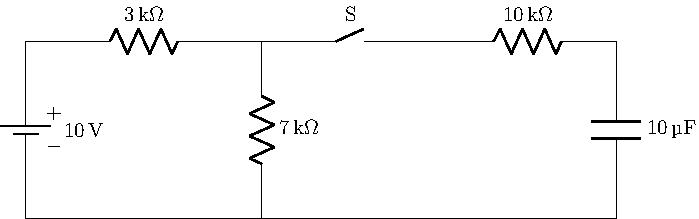
\includegraphics[width = \columnwidth]{figs/c_fig1.pdf}
\end{figure}
\\
\solution
\\
For $t \ge 0$:
\begin{figure}[h!]
    \centering
    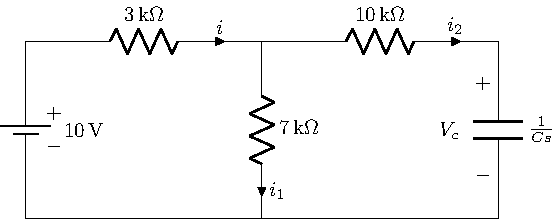
\includegraphics[width=\columnwidth]{figs/c_fig2.pdf}
\end{figure}

In steady state, no current flows through capacitor.
\begin{align}
i_2 &= 0 \\
\implies i &= i_1 \\
V &= (7\text{k}\ohm)(i_1) \\
10\text{V} &= (10\text{k}\ohm)(i_1) \\
\implies i_1 &= 1\text{mA} \\
V &= 7\text{V}
\end{align}
\end{document}